\documentclass[../diss.tex]{subfiles}

\begin{document}

In this chapter, I will describe all the work completed before any code was written. This includes: the underlying theory (\cref{sec:gctheory}), a requirements analysis (\cref{sec:requirements}), my choice of tools (\cref{sec:tools}), the software engineering techniques used (\cref{sec:softwareengineering}) and the starting point (\cref{sec:startingpoint}).

\section{Garbage Collection} \label{sec:gctheory}

Garbage collection is a form of automatic memory management commonly used within programming languages. Semantic garbage refers to memory allocated by the program which will no longer be used although it may still be accessible. Syntactic garbage is an approximation to semantic garbage, it considers anything that cannot be accessed by the program as garbage. Computing the set of semantic garbage is undecidable because it requires future knowledge of the program execution, therefore we must use syntactic garbage. This is safe, in the sense that the garbage collector will not collect live objects, because syntactic garbage is a subset of semantic garbage.

The user program is known as the mutator because it is the part of the overall system which allocates and modifies objects. The collector is the part which runs a garbage collection algorithm.

Garbage collection algorithms tend to be one of two types: reference counting or tracing collectors. Reference counting collectors\cite{referencecounting} track the number of pointers to each object, when the count becomes 0 the object is removed. The main problem with this approach is that cyclic data-structures are not seen as garbage. Tracing collectors, such as the mark and sweep algorithm, are based on the idea of reachability from a set of starting objects, called the root set. The root set consists of the stack, registers and global data regions which can all contain pointers to objects on the heap. See \cite{overview} for an overview of garbage collection algorithms and \cite{terms} for an overview of garbage collection terms.

% Reference memorymanagement.org for details on other terms?

\subsection{Mark and Sweep Garbage Collection} \label{sec:markandsweep}

Mark and Sweep is a kind of tracing garbage collection algorithm that is composed of two phases. The mark phase simply performs a search from the root set and marks everything that is reachable. The sweep phase looks at each object and removes those that are unmarked. Over time the heap can become fragmented which can be solved by compacting the heap and updating any pointers to those objects. Compaction is the process of moving objects so that there is no dead space between them. Figure \ref{fig:markandsweepcollection} shows an example mark and sweep collection without compaction.

\begin{figure}
    \centering
    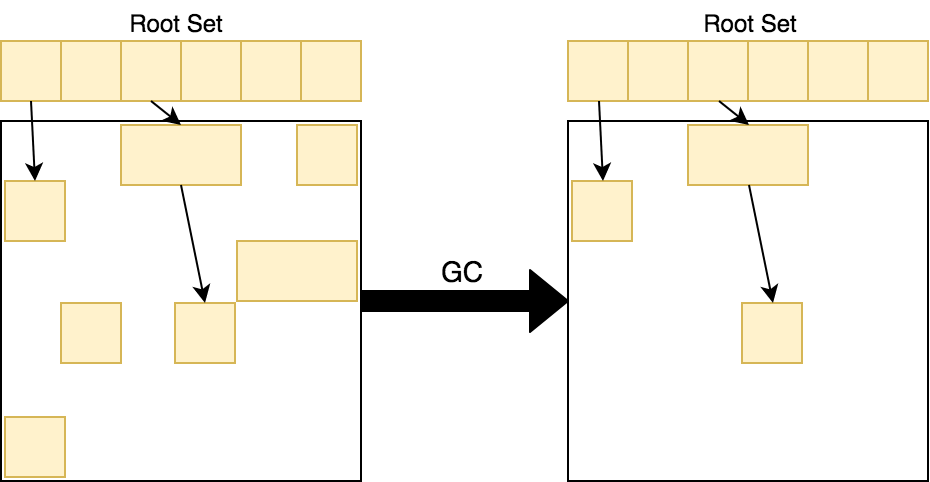
\includegraphics[max width=\linewidth]{figs/markandsweep.png}
    \caption{Mark and sweep collection without compaction}
    \label{fig:markandsweepcollection}
\end{figure}

\subsection{Copying Garbage Collection}

Copying garbage collection\cite{copyingcollector} is another form of tracing garbage collection. It splits the heap into two sections: one is used by the program (active heap) and the other is reserved for use during collection. Memory is only allocated to the user program from the active heap. When the garbage collector runs, reachable data is copied from the active heap to the other. Everything in the active heap is removed and the two heaps switch roles. Fragmentation is handled automatically as the copied objects are placed in contiguous memory locations which can be seen in Figure \ref{fig:copyingcollection}. The major disadvantage is that only half of the system's memory can be used by the program.

\begin{figure}
    \centering
    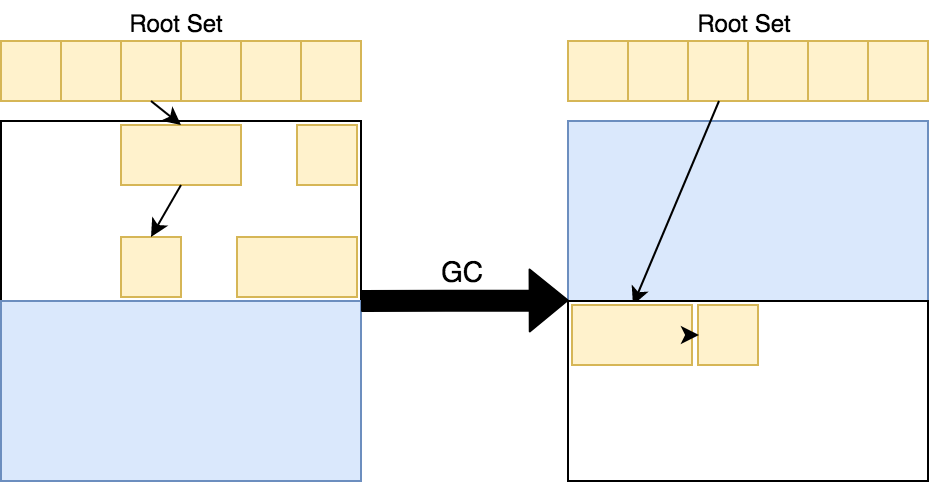
\includegraphics[max width=\linewidth]{figs/copycollection.png}
    \caption{Copying Collection}
    \label{fig:copyingcollection}
\end{figure}

\subsection{Generational Garbage Collection} \label{sec:generationalgarbagecollection}
% Explain this section a lot more

My project uses the generational garbage collection algorithm\cite{generational}, which is based on the assumption that most objects die shortly after being allocated. Another way to think about this is that an object which has survived many collections has a high probability of being a long-lived object, and because of this we do not need to consider it for collection every time.

The generational algorithm works by segregating the heap into generations, which contain objects of similar age. When collecting, the garbage collector will check younger generations more frequently than older ones. If an object survives collection it is promoted into the next generation (unless already in the oldest generation). Sometimes, different collection algorithms are used on the new and old generations. A common scenario for a garbage collector with $N$ generations is to use a copy collector for the youngest $N-1$ generations and mark and sweep for the oldest one. The reason for this is that copy collection gives us the promotion step and defragmentation without any extra processing.

The benefit of the generational algorithm is that each collection should be faster as the number of objects it has to consider is lower when compared to a mark and sweep garbage collector. In the latter, this can lead to a visible pause which is undesirable. There are limits to the generational algorithm, in particular it is not always comprehensive (it may fail to collect all the garbage). An example of this can be seen in Figure \ref{fig:generational} where an object is referenced by an older object which itself is garbage. When not collecting older objects they are treated as live. This does not mean that garbage left behind after one collection will not be collected in another.

\begin{figure}
    \centering
    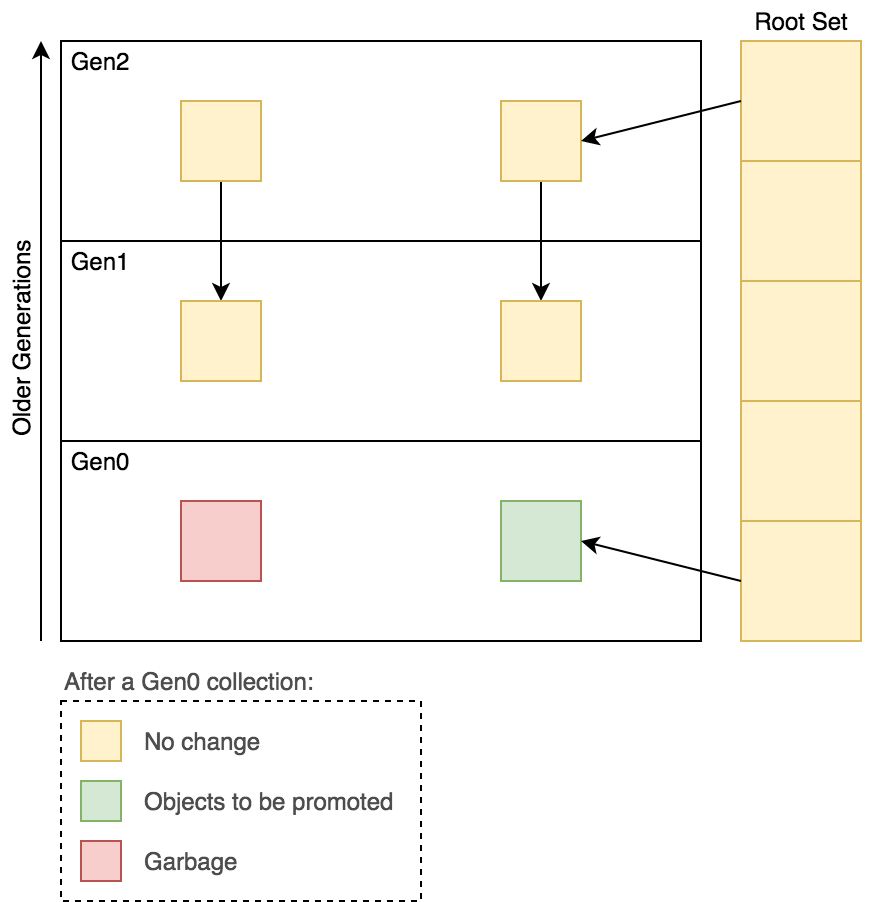
\includegraphics[max width=\linewidth]{figs/generational.png}
    \caption{Example heap layout when using a generational garbage collector}
    \label{fig:generational}
\end{figure}

\subsection{Write Barriers} \label{sec:prepwritebarriers}

A write-barrier\cite{writebarriers} intercepts writes to certain memory locations, therefore allowing the program to track changes to the memory. Depending on the implementation the write may or may not occur, but for garbage collection we allow the write to happen. Garbage collectors rely on knowing what references are contained within each object. The generational algorithm only considers objects in specific generations each time, the write-barrier allows it to know if an object is referenced by an older object. Some studies show the number of older to younger references to be less than 1\% of all references. However, without knowing that these pointers exist we risk collecting live objects.

One way of implementing a write-barrier is to insert a small thunk before every pointer assignment which records in a card-table that a particular block of memory is dirty. When collecting we include every object in a dirty block of memory as being a root. This requires compiler support to insert the thunk before every pointer assignment and therefore is unsuitable for my solution. Most operating systems allow permissions to be specified for parts of the memory. This can be used to implement a write-barrier in software by marking blocks of memory as read-only and trapping the resultant segmentation fault. This is the approach used by my garbage collector, \cref{sec:writebarrier} provides the implementation details.

\subsection{Conservative Collection} \label{lab:conservative}

Conservative collection\cite{conservative} is useful for adding garbage collection to a programming language which never intended to have it as a feature. When we are in an environment where it is not possible to know which values are references, we make the conservative decision to threat any value which \emph{might} be a pointer as a reference. Figure \ref{fig:conservative} shows an example of this conservative decision. The drawback of this approach is that we may find a value which looks like a pointer to an object but in actual fact it was just a numerical value. It is not possible to implement a full copying collector that is conservative. A copying collector moves the objects to new locations which requires updating the references to them, but we do not know for sure that the value was a pointer thus the update operation is not safe. Another implication of this is that we cannot perform compaction to remove fragmentation for the same reasons.

\begin{figure}
    \centering
    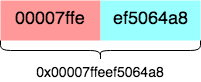
\includegraphics{figs/conservative.png}
    \caption{Showing how two integers may be considered as a single pointer}
    \label{fig:conservative}
\end{figure}

\subsection{Multi-threaded Garbage Collection} \label{sec:multithreadingmodels}

Many real-world applications deal with multiple threads of execution and so a garbage collector which works with only a single thread is not very useful. There are many different algorithms that can be used, the main techniques are discussed here and the implementation that my garbage collector uses is discussed.

A stop-the-world garbage collector does not allow the mutator to run during garbage collection. If the mutator consists of multiple threads then these must all be halted before the garbage collector can run. This approach is the simplest because new objects cannot be created and objects do not become unreachable while the collector is running. When implementing this type of garbage collector, it is easier to guarantee that data will not end up in an inconsistent state.

An alternative approach is to use an incremental garbage collector. This performs a small amount of garbage collection in discrete intervals. This type is preferred when the software must guarantee response times such as in user interfaces. However, the time to complete a collection (which is the sum of many smaller quanta) is greater than that for the stop-the-world approach due to the fact it must avoid data inconsistencies. 

To take this further we can have a parallel collector (also known as a concurrent collector) which executes simultaneously with the mutator. A problem with this approach is that the mutator can change objects while collection is occurring.

Although it was not planned to be thread-safe initially, I added this feature as part of an extension to the project. It involved a preparation stage despite the fact that a large amount of the work had already been completed. This ties into the software engineering techniques used during the implementation and my chosen approach allowed the development of the extension to run smoothly (\cref{sec:softwareengineering}). I chose a stop-the-world implementation because it is simpler to implement and therefore it would be easier to meet the project deadlines. In addition, it is simpler to test and evaluate in a convincing way.

\section{Requirements Analysis} \label{sec:requirements}

Having looked at the basics of generational and conservative collection, we can consider the project requirements. Here I will also discuss the requirements of the thread-safety extension. These are closely linked to the success criteria from the initial proposal (Appendix \ref{appendix:initialproposal}). Table \ref{tab:requirements} provides a high-level summary of all the requirements.

\subsubsection{Allocation}

It is important that the main program be able to allocate memory. For garbage collection to work as expected it needed to know what objects have previously been allocated and contain some meta-data for each one. This ties into the first success criterion: \emph{``produce a garbage collector which never collects a live object''}. Efficient data-structures were implemented to contain the required information to give the best possible performance. Another implication of the first success criterion is that it needed a method of finding objects with pointers to other objects. To achieve this I implemented a write-barrier which tracks writes to the allocated objects and therefore allows the garbage collector to inspect the contents for pointers. These requirements were of high priority due to the close relation to the success criteria.

Fragmentation was also a concern for long-running programs, I previously stated that an explicit compaction step is not possible in a conservative collector. This was a low priority requirement because machines with sufficient memory can tolerate small amounts of fragmentation.

\subsubsection{Collection}

To be able to perform a collection, the garbage collector needed to identify pointers from the root set. Global roots were not considered although it is mentioned in the future work section (\cref{sec:futurework}).

The second success criterion states that \emph{``the garbage collector should run when when the number of objects in a generation passes a threshold [...]''}. To achieve this the garbage collector had to store runtime statistics so that it can determine when to run. These statistics were also used in the evaluation section of this dissertation.

\subsubsection{Multi-threading}

To be able to coordinate the collection (recall that it uses a stop-the-world approach) the garbage collector needed to store information about each thread. Every thread has its own stack, whose location must be known to compute the root set. Mutual exclusion was critical to protect concurrent access to shared variables. At different stages of the collection, threads have to wait for a condition to be true or signal that some work was completed. It uses condition variables for each of the stages so that threads can communicate. These requirements are not critical as they are part of an extension to the project however they are of high risk as bugs in the code could break the garbage collector.

\begin{table}
    \centering
    \begin{tabular}{| l | l | l | l |}
        \hline
         \bf{Requirement} & \bf{Priority} & \bf{Risk} & \bf{Difficulty} \\ \hline
         Track allocated objects & High & High & Medium \\ \hline
         Implement a write-barrier & High & High & Hard \\ \hline
         Store object generation meta-data & High & High & Low \\ \hline
         Handle fragmentation & Low & Low & Hard \\ \hline
         Search the stack for roots & High & High & Medium \\ \hline
         Search registers for roots & High & High & Medium \\ \hline
         Search global data regions for roots & Low & Low & Medium \\ \hline
         Store per-thread meta-data & High & High & Low \\ \hline
         Use mutual exclusion to protect access to shared variables & Medium & High & Medium \\ \hline
         Use condition variables for communication & Medium & High & Medium \\ \hline
    \end{tabular}
    \caption{Table of high-level requirements}
    \label{tab:requirements}
\end{table}

\section{Choice of Tools} \label{sec:tools}

In this section I will discuss my development environment and the tools which I used to develop my garbage collector. I am using a MacBook Pro with an Intel Core i7 processor clocked at 2.5GHz, running High Sierra (version 10.13.1). It is important to note the development platform as results in different environments may differ.

Naturally, C was chosen as my primary programming language and C++ for writing my unit tests. C++ is used because so that I can make use of C++ testing frameworks. The testing framework of choice was Catch since this is a header-only framework which is simple to use while being very powerful. 

I used Git for revision control which is of key importance for large projects. I used BitBucket for hosting which also acts as my primary backup. At the end of every week I also created a copy of the progress to a memory pen. Matlab and LaTeX are also used to produce graphs for evaluation and for producing the corresponding documentation respectively.

It was important to ensure that the use of the listed software was allowed under the specified licences before starting any work. As I am releasing my solution as open-source software with an MIT licence it can be adequately described as `non-commercial'. Many of the libraries used have open-source licences such as the APSL, University of Illinois/NCSA, BSDv3, GPLv2 and Boost Software Licence 1.0. All of these allow the creation of my garbage collector with the common limitation that the creators cannot be held liable for any damages. Matlab and CLion have proprietary licences, I am specifically using the student versions of these pieces of software. The licences specify that these can be used for non-commercial projects and therefore are suitable for my purposes.

\begin{table}
    \centering
    \begin{tabular}{|l|l|l|l|}
        \hline
        \bf{Tool} & \bf{Version} & \bf{Licence} & \bf{Purpose} \\ \hline
        macOS & 10.13.1 & APSL & Operating System \\ \hline
        Clang & 900.0.39.2 & University of Illinois/NCSA & Compiler \\ \hline
        Clion & 2017.2.1 & Proprietary, Student Licence & IDE \\ \hline
        CMake & 3.8 & BSDv3 & Build Tool \\ \hline
        lldb & 360.99.0 & University of Illinois/NCSA & Debugger \\ \hline
        Valgrind & 3.13.0 & GPLv2 & Debugging \\ \hline
        Git & 2.13.3 & GPLv2 & Revision Control \\ \hline
        Catch & 1.10.0 & Boost Software Licence 1.0 & Unit Testing Framework \\ \hline
        MatLab & 9.3 & Proprietary, Student Licence & Evaluation \\ \hline
    \end{tabular}
    \caption{All tools used in development}
    \label{tab:tools}
\end{table}

\section{Software Engineering Techniques} \label{sec:softwareengineering}

I adopted an Iterative and Incremental Development Model for this project. This allows any problems to be detected and dealt with earlier than other development models, which is crucial for producing a successful project within the limited time. This model also allowed me to use what was learned in earlier parts of the development to my advantage.

I also use abstraction and modularisation in certain parts of the project which allows them to be developed and tested in isolation. This can be seen in the Allocator and Threads modules of the projects and provides the advantage that they can easily be changed for alternative implementations in the future. 

Proper commenting was used to annotate function definition which increases the readability of the code. I keep a consistent form of comment throughout the project as seen in Listing \ref{lst:comment}.

\begin{figure*}
\begin{lstlisting}[caption=Function comment example, label={lst:comment}]
/*
 * Function Name
 * -----------------------
 * Description
 *
 * Inputs
 *
 * Returns
 */
\end{lstlisting}
\end{figure*}

\section{Starting Point} \label{sec:startingpoint}

\begin{table}
    \centering
    \begin{tabular}{| p{5cm} | p{10cm} |}
        \hline
        \bf{Course} & \bf{Application} \\ \hline
        Computer Design & Understanding memory management and signal handling \\ \hline
        Programming in C and C++ & Primary programming language \\ \hline
        Concurrent and Distributed Systems & Multi-threading extension \\ \hline
        Software Engineering & Proper software engineering practices \\ \hline
        Compiler Construction & Garbage collection algorithms \\ \hline
    \end{tabular}
    \caption{Applicability of the CS Tripos}
    \label{tab:tripos}
\end{table}

The Computer Science Tripos has been very applicable to this project as highlighted in Table \ref{tab:tripos}. However further research into garbage collection theory has been required for this project. This was achieved using various online resources and the Boehm GC for inspiration.

\section{Summary}

In this chapter, I have discussed the work completed before the implementation began. I have discussed the theory in detail, and the goals of the project, as well as the tools and techniques used. The following chapter gives details about how this design was implemented.

\end{document}